\documentclass[12pt,a4paper]{article}

% ==========================================================
% PAQUETES
% ==========================================================
\usepackage[utf8]{inputenc}
\usepackage[T1]{fontenc}
\usepackage[spanish,es-tabla]{babel}
\usepackage{amsmath, amssymb, amsfonts}
\usepackage{geometry}
\usepackage{array}
\usepackage{booktabs}
\usepackage{enumitem}
\usepackage{xcolor}
\usepackage{fancyhdr}
\usepackage{hyperref}
\usepackage{listings}
\usepackage{tcolorbox}
\usepackage{titlesec}
\usepackage{setspace}
\usepackage{graphicx}
\usepackage{float}
\usepackage{caption}

% ==========================================================
% CONFIGURACIÓN GENERAL
% ==========================================================
\geometry{
    top=2.5cm,
    bottom=2.5cm,
    left=2.5cm,
    right=2.5cm
}

\setstretch{1.15}
\setlength{\parindent}{0pt}
\setlength{\parskip}{6pt}
\setlength{\headheight}{15pt}
\graphicspath{{figures/}}

\definecolor{azulunsaac}{RGB}{20,63,112}
\definecolor{grisclaro}{RGB}{245,247,250}
\definecolor{grisoscuro}{RGB}{55,65,81}

\hypersetup{
    colorlinks=true,
    linkcolor=azulunsaac,
    urlcolor=azulunsaac,
    citecolor=azulunsaac
}

\titleformat{\section}
{\Large\bfseries\color{azulunsaac}}
{\thesection.}{0.5em}{}

\titleformat{\subsection}
{\large\bfseries\color{grisoscuro}}
{\thesubsection.}{0.5em}{}

\pagestyle{fancy}
\fancyhf{}
\lhead{IF460AIN -- Computación Cuántica}
\rhead{Laboratorio 6}
\cfoot{\thepage}

% ==========================================================
% COMANDOS
% ==========================================================
\newcommand{\ket}[1]{\left|#1\right\rangle}
\newcommand{\bra}[1]{\left\langle#1\right|}
\newcommand{\braket}[2]{\left\langle #1 \middle| #2 \right\rangle}
\newcommand{\colvec}[2]{\begin{pmatrix} #1 \\ #2 \end{pmatrix}}

\newtcolorbox{resultado}{
    colback=grisclaro,
    colframe=azulunsaac,
    arc=2mm,
    boxrule=0.8pt,
    title=Resultado,
    fonttitle=\bfseries
}

\lstdefinestyle{pythonstyle}{
    language=Python,
    basicstyle=\ttfamily\small,
    keywordstyle=\bfseries\color{azulunsaac},
    commentstyle=\itshape\color{gray},
    stringstyle=\color{teal},
    showstringspaces=false,
    breaklines=true,
    frame=single,
    rulecolor=\color{gray},
    backgroundcolor=\color{grisclaro},
    tabsize=4
}

\lstset{style=pythonstyle}

% ==========================================================
% DOCUMENTO
% ==========================================================
\begin{document}

% ==========================================================
% PORTADA
% ==========================================================
\begin{titlepage}
    \centering

    \vspace*{1cm}

    {\Large \textbf{UNIVERSIDAD NACIONAL DE SAN ANTONIO ABAD DEL CUSCO}}\\[0.4cm]
    {\large Facultad de Ingeniería Eléctrica, Electrónica, Informática y Mecánica}\\[0.2cm]
    {\large Escuela Profesional de Ingeniería Informática y de Sistemas}\\[1.5cm]

    {\Huge \textbf{Laboratorio 6}}\\[0.4cm]
    {\LARGE \textbf{Circuitos Cuánticos y Esfera de Bloch}}\\[1.2cm]

    \begin{tcolorbox}[
        colback=grisclaro,
        colframe=azulunsaac,
        width=0.85\textwidth,
        arc=2mm,
        boxrule=0.8pt
    ]
    \begin{tabular}{>{\bfseries}p{4.2cm} p{8cm}}
        Curso: & IF460AIN -- Computación Cuántica \\
        Docente: & Raúl Huillca Huallparimachi \\
        Estudiante: & Edmil Jampier Saire Bustamante \\
        Código: & 174449 \\
        Evaluación: & Laboratorio 6 \\
    \end{tabular}
    \end{tcolorbox}

    \vfill

    {\large Cusco -- Perú}\\[0.2cm]
    {\large \today}

\end{titlepage}

\tableofcontents
\newpage

% ==========================================================
\section{Representación del Qubit}

Sea el estado:

\[
\ket{\psi}=\cos\frac{\theta}{2}\ket{0}+e^{i\lambda}\sin\frac{\theta}{2}\ket{1}
\]

Un qubit general se expresa como:

\[
\ket{\psi}=\alpha\ket{0}+\beta\ket{1}
\]

Por comparación directa, se obtiene:

\[
\alpha=\cos\frac{\theta}{2}
\]

\[
\beta=e^{i\lambda}\sin\frac{\theta}{2}
\]

\begin{resultado}
\[
\boxed{\alpha=\cos\frac{\theta}{2}}
\qquad
\boxed{\beta=e^{i\lambda}\sin\frac{\theta}{2}}
\]
\end{resultado}

\subsection{Verificación de la normalización}

Para que un estado cuántico sea físicamente válido, debe cumplir:

\[
|\alpha|^2+|\beta|^2=1
\]

Calculamos cada término:

\[
|\alpha|^2=\left|\cos\frac{\theta}{2}\right|^2=\cos^2\frac{\theta}{2}
\]

\[
|\beta|^2=\left|e^{i\lambda}\sin\frac{\theta}{2}\right|^2
\]

Como el módulo de una fase compleja es igual a uno:

\[
|e^{i\lambda}|=1
\]

Entonces:

\[
|\beta|^2=|e^{i\lambda}|^2\left|\sin\frac{\theta}{2}\right|^2
\]

\[
|\beta|^2=\sin^2\frac{\theta}{2}
\]

Sumando:

\[
|\alpha|^2+|\beta|^2
=
\cos^2\frac{\theta}{2}
+
\sin^2\frac{\theta}{2}
\]

Por la identidad trigonométrica fundamental:

\[
\cos^2 x+\sin^2 x=1
\]

se concluye:

\[
|\alpha|^2+|\beta|^2=1
\]

\begin{resultado}
El estado está correctamente normalizado.
\[
\boxed{|\alpha|^2+|\beta|^2=1}
\]
\end{resultado}

\subsection{Significado físico de \texorpdfstring{$\theta$}{theta} y \texorpdfstring{$\lambda$}{lambda}}

El parámetro \(\theta\) determina la posición del qubit respecto al eje vertical de la esfera de Bloch. Además, controla las probabilidades de obtener \(\ket{0}\) o \(\ket{1}\) al medir en la base computacional.

\[
P(0)=|\alpha|^2=\cos^2\frac{\theta}{2}
\]

\[
P(1)=|\beta|^2=\sin^2\frac{\theta}{2}
\]

El parámetro \(\lambda\) representa la fase relativa entre las componentes \(\ket{0}\) y \(\ket{1}\). Esta fase no altera directamente las probabilidades de medición en la base computacional, pero sí influye en los fenómenos de interferencia y en el resultado de aplicar compuertas cuánticas.

\begin{resultado}
\[
\theta \text{ controla las probabilidades de medición.}
\]
\[
\lambda \text{ controla la fase relativa entre } \ket{0} \text{ y } \ket{1}.
\]
\end{resultado}

% ==========================================================
\section{Coordenadas de la Esfera de Bloch}

Para el estado:

\[
\ket{\psi}=\cos\frac{\theta}{2}\ket{0}+e^{i\lambda}\sin\frac{\theta}{2}\ket{1}
\]

se tiene:

\[
\alpha=\cos\frac{\theta}{2}
\]

\[
\beta=e^{i\lambda}\sin\frac{\theta}{2}
\]

Las coordenadas de Bloch son:

\[
x=2\operatorname{Re}(\alpha^*\beta)
\]

\[
y=2\operatorname{Im}(\alpha^*\beta)
\]

\[
z=|\alpha|^2-|\beta|^2
\]

\subsection{Demostración de la coordenada \texorpdfstring{$z$}{z}}

\[
z=|\alpha|^2-|\beta|^2
\]

Sustituyendo las amplitudes:

\[
z=
\left|\cos\frac{\theta}{2}\right|^2
-
\left|e^{i\lambda}\sin\frac{\theta}{2}\right|^2
\]

\[
z=
\cos^2\frac{\theta}{2}
-
\sin^2\frac{\theta}{2}
\]

Usando la identidad:

\[
\cos^2 a-\sin^2 a=\cos(2a)
\]

con:

\[
a=\frac{\theta}{2}
\]

resulta:

\[
z=\cos\theta
\]

\begin{resultado}
\[
\boxed{z=|\alpha|^2-|\beta|^2=\cos\theta}
\]
\end{resultado}

\subsection{Demostración de la coordenada \texorpdfstring{$x$}{x}}

\[
x=2\operatorname{Re}(\alpha^*\beta)
\]

Como:

\[
\alpha=\cos\frac{\theta}{2}
\]

entonces:

\[
\alpha^*=\cos\frac{\theta}{2}
\]

Por lo tanto:

\[
\alpha^*\beta=
\cos\frac{\theta}{2}
\cdot
e^{i\lambda}\sin\frac{\theta}{2}
\]

\[
\alpha^*\beta=
\cos\frac{\theta}{2}
\sin\frac{\theta}{2}
e^{i\lambda}
\]

Multiplicando por 2:

\[
2\alpha^*\beta=
2\cos\frac{\theta}{2}
\sin\frac{\theta}{2}
e^{i\lambda}
\]

Como:

\[
2\sin a\cos a=\sin(2a)
\]

se obtiene:

\[
2\alpha^*\beta=\sin\theta e^{i\lambda}
\]

Usando la fórmula de Euler:

\[
e^{i\lambda}=\cos\lambda+i\sin\lambda
\]

entonces:

\[
2\alpha^*\beta
=
\sin\theta(\cos\lambda+i\sin\lambda)
\]

La parte real es:

\[
x=\sin\theta\cos\lambda
\]

\begin{resultado}
\[
\boxed{x=2\operatorname{Re}(\alpha^*\beta)=\sin\theta\cos\lambda}
\]
\end{resultado}

\subsection{Demostración de la coordenada \texorpdfstring{$y$}{y}}

\[
y=2\operatorname{Im}(\alpha^*\beta)
\]

Del desarrollo anterior:

\[
2\alpha^*\beta
=
\sin\theta(\cos\lambda+i\sin\lambda)
\]

La parte imaginaria es:

\[
y=\sin\theta\sin\lambda
\]

\begin{resultado}
\[
\boxed{y=2\operatorname{Im}(\alpha^*\beta)=\sin\theta\sin\lambda}
\]
\end{resultado}

\subsection{Interpretación de cada coordenada}

La esfera de Bloch representa geométricamente el estado de un qubit puro mediante un vector unitario:

\[
(x,y,z)
\]

donde:

\begin{itemize}
    \item \(z\) mide la diferencia entre las probabilidades de \(\ket{0}\) y \(\ket{1}\).
    \item \(x\) representa la coherencia real entre las amplitudes del estado.
    \item \(y\) representa la coherencia imaginaria asociada a la fase relativa.
\end{itemize}

Estados importantes:

\[
\ket{0}\rightarrow(0,0,1)
\]

\[
\ket{1}\rightarrow(0,0,-1)
\]

\[
\frac{\ket{0}+\ket{1}}{\sqrt{2}}\rightarrow(1,0,0)
\]

\[
\frac{\ket{0}+i\ket{1}}{\sqrt{2}}\rightarrow(0,1,0)
\]

% ==========================================================
\section{Compuertas Cuánticas}

Se definen los estados base:

\[
\ket{0}=
\begin{pmatrix}
1\\
0
\end{pmatrix}
\qquad
\ket{1}=
\begin{pmatrix}
0\\
1
\end{pmatrix}
\]

\subsection{Compuerta X}

La compuerta \(X\) está definida como:

\[
X=
\begin{pmatrix}
0 & 1\\
1 & 0
\end{pmatrix}
\]

\subsubsection*{Cálculo de \texorpdfstring{$X\ket{0}$}{X ket 0}}

\[
X\ket{0}
=
\begin{pmatrix}
0 & 1\\
1 & 0
\end{pmatrix}
\begin{pmatrix}
1\\
0
\end{pmatrix}
\]

\[
X\ket{0}
=
\begin{pmatrix}
0\\
1
\end{pmatrix}
=
\ket{1}
\]

\begin{resultado}
\[
\boxed{X\ket{0}=\ket{1}}
\]
\end{resultado}

\subsubsection*{Cálculo de \texorpdfstring{$X\ket{1}$}{X ket 1}}

\[
X\ket{1}
=
\begin{pmatrix}
0 & 1\\
1 & 0
\end{pmatrix}
\begin{pmatrix}
0\\
1
\end{pmatrix}
\]

\[
X\ket{1}
=
\begin{pmatrix}
1\\
0
\end{pmatrix}
=
\ket{0}
\]

\begin{resultado}
\[
\boxed{X\ket{1}=\ket{0}}
\]
\end{resultado}

\subsubsection*{Interpretación}

La compuerta \(X\) actúa como una compuerta NOT cuántica. Intercambia los estados base:

\[
\ket{0}\leftrightarrow\ket{1}
\]

En la esfera de Bloch, equivale a una rotación de \(180^\circ\) alrededor del eje \(x\).

\subsection{Compuerta Z}

La compuerta \(Z\) está definida como:

\[
Z=
\begin{pmatrix}
1 & 0\\
0 & -1
\end{pmatrix}
\]

\subsubsection*{Cálculo de \texorpdfstring{$Z\ket{0}$}{Z ket 0}}

\[
Z\ket{0}
=
\begin{pmatrix}
1 & 0\\
0 & -1
\end{pmatrix}
\begin{pmatrix}
1\\
0
\end{pmatrix}
\]

\[
Z\ket{0}
=
\begin{pmatrix}
1\\
0
\end{pmatrix}
=
\ket{0}
\]

\begin{resultado}
\[
\boxed{Z\ket{0}=\ket{0}}
\]
\end{resultado}

\subsubsection*{Cálculo de \texorpdfstring{$Z\ket{1}$}{Z ket 1}}

\[
Z\ket{1}
=
\begin{pmatrix}
1 & 0\\
0 & -1
\end{pmatrix}
\begin{pmatrix}
0\\
1
\end{pmatrix}
\]

\[
Z\ket{1}
=
\begin{pmatrix}
0\\
-1
\end{pmatrix}
=
-\ket{1}
\]

\begin{resultado}
\[
\boxed{Z\ket{1}=-\ket{1}}
\]
\end{resultado}

\subsubsection*{Efecto de fase}

La compuerta \(Z\) deja intacta la componente \(\ket{0}\), pero multiplica la componente \(\ket{1}\) por \(-1\). Como:

\[
-1=e^{i\pi}
\]

se interpreta que \(Z\) introduce una fase relativa de \(\pi\) en la componente \(\ket{1}\).

\subsection{Compuerta S}

La compuerta \(S\) está definida como:

\[
S=
\begin{pmatrix}
1 & 0\\
0 & i
\end{pmatrix}
\]

\subsubsection*{Cálculo de \texorpdfstring{$S\ket{0}$}{S ket 0}}

\[
S\ket{0}
=
\begin{pmatrix}
1 & 0\\
0 & i
\end{pmatrix}
\begin{pmatrix}
1\\
0
\end{pmatrix}
\]

\[
S\ket{0}
=
\begin{pmatrix}
1\\
0
\end{pmatrix}
=
\ket{0}
\]

\begin{resultado}
\[
\boxed{S\ket{0}=\ket{0}}
\]
\end{resultado}

\subsubsection*{Cálculo de \texorpdfstring{$S\ket{1}$}{S ket 1}}

\[
S\ket{1}
=
\begin{pmatrix}
1 & 0\\
0 & i
\end{pmatrix}
\begin{pmatrix}
0\\
1
\end{pmatrix}
\]

\[
S\ket{1}
=
\begin{pmatrix}
0\\
i
\end{pmatrix}
=
i\ket{1}
\]

\begin{resultado}
\[
\boxed{S\ket{1}=i\ket{1}}
\]
\end{resultado}

\subsubsection*{Demostración de \texorpdfstring{$i=e^{i\pi/2}$}{i=e^ipi/2}}

Por la fórmula de Euler:

\[
e^{ix}=\cos x+i\sin x
\]

Para:

\[
x=\frac{\pi}{2}
\]

se tiene:

\[
e^{i\pi/2}
=
\cos\frac{\pi}{2}
+
i\sin\frac{\pi}{2}
\]

\[
e^{i\pi/2}=0+i(1)
\]

\[
e^{i\pi/2}=i
\]

\begin{resultado}
\[
\boxed{i=e^{i\pi/2}}
\]
\end{resultado}

% ==========================================================
\section{Compuerta Hadamard}

La compuerta Hadamard está definida como:

\[
H=
\frac{1}{\sqrt{2}}
\begin{pmatrix}
1 & 1\\
1 & -1
\end{pmatrix}
\]

\subsection{Cálculo de \texorpdfstring{$H\ket{0}$}{H ket 0}}

\[
H\ket{0}
=
\frac{1}{\sqrt{2}}
\begin{pmatrix}
1 & 1\\
1 & -1
\end{pmatrix}
\begin{pmatrix}
1\\
0
\end{pmatrix}
\]

\[
H\ket{0}
=
\frac{1}{\sqrt{2}}
\begin{pmatrix}
1\\
1
\end{pmatrix}
\]

\[
H\ket{0}
=
\frac{1}{\sqrt{2}}\ket{0}
+
\frac{1}{\sqrt{2}}\ket{1}
\]

\begin{resultado}
\[
\boxed{H\ket{0}=\frac{\ket{0}+\ket{1}}{\sqrt{2}}}
\]
\end{resultado}

Este estado se conoce como:

\[
\ket{+}=\frac{\ket{0}+\ket{1}}{\sqrt{2}}
\]

\subsection{Cálculo de \texorpdfstring{$H\ket{1}$}{H ket 1}}

\[
H\ket{1}
=
\frac{1}{\sqrt{2}}
\begin{pmatrix}
1 & 1\\
1 & -1
\end{pmatrix}
\begin{pmatrix}
0\\
1
\end{pmatrix}
\]

\[
H\ket{1}
=
\frac{1}{\sqrt{2}}
\begin{pmatrix}
1\\
-1
\end{pmatrix}
\]

\[
H\ket{1}
=
\frac{1}{\sqrt{2}}\ket{0}
-
\frac{1}{\sqrt{2}}\ket{1}
\]

\begin{resultado}
\[
\boxed{H\ket{1}=\frac{\ket{0}-\ket{1}}{\sqrt{2}}}
\]
\end{resultado}

Este estado se conoce como:

\[
\ket{-}=\frac{\ket{0}-\ket{1}}{\sqrt{2}}
\]

\subsection{Interpretación del concepto de superposición}

La superposición es una propiedad cuántica que permite que un qubit se encuentre en una combinación lineal de los estados base \(\ket{0}\) y \(\ket{1}\).

Por ejemplo:

\[
H\ket{0}=
\frac{\ket{0}+\ket{1}}{\sqrt{2}}
\]

Al medir este estado en la base computacional, las probabilidades son:

\[
P(0)=\left|\frac{1}{\sqrt{2}}\right|^2=\frac{1}{2}
\]

\[
P(1)=\left|\frac{1}{\sqrt{2}}\right|^2=\frac{1}{2}
\]

Por tanto, existe un \(50\%\) de probabilidad de medir \(\ket{0}\) y un \(50\%\) de probabilidad de medir \(\ket{1}\).

% ==========================================================
\section{Circuitos Cuánticos}

\subsection{Circuito \texorpdfstring{$\ket{0}\rightarrow H\rightarrow Z$}{ket 0 H Z}}

Primero se aplica la compuerta \(H\) sobre \(\ket{0}\):

\[
H\ket{0}=
\frac{\ket{0}+\ket{1}}{\sqrt{2}}
\]

Luego se aplica la compuerta \(Z\):

\[
Z\left(
\frac{\ket{0}+\ket{1}}{\sqrt{2}}
\right)
=
\frac{Z\ket{0}+Z\ket{1}}{\sqrt{2}}
\]

Como:

\[
Z\ket{0}=\ket{0}
\]

\[
Z\ket{1}=-\ket{1}
\]

entonces:

\[
\frac{Z\ket{0}+Z\ket{1}}{\sqrt{2}}
=
\frac{\ket{0}-\ket{1}}{\sqrt{2}}
\]

\begin{resultado}
\[
\boxed{
\ket{0}\xrightarrow{H}\xrightarrow{Z}
\frac{\ket{0}-\ket{1}}{\sqrt{2}}
}
\]
\end{resultado}

El estado final es:

\[
\ket{-}=\frac{\ket{0}-\ket{1}}{\sqrt{2}}
\]

\subsubsection*{Interpretación}

La compuerta \(H\) crea una superposición equilibrada. Luego, \(Z\) introduce una fase negativa en la componente \(\ket{1}\). El vector de Bloch pasa del eje \(x\) positivo al eje \(x\) negativo:

\[
(1,0,0)\rightarrow(-1,0,0)
\]

\subsection{Circuito \texorpdfstring{$\ket{0}\rightarrow H\rightarrow S$}{ket 0 H S}}

Primero se aplica \(H\):

\[
H\ket{0}=
\frac{\ket{0}+\ket{1}}{\sqrt{2}}
\]

Luego se aplica \(S\):

\[
S\left(
\frac{\ket{0}+\ket{1}}{\sqrt{2}}
\right)
=
\frac{S\ket{0}+S\ket{1}}{\sqrt{2}}
\]

Como:

\[
S\ket{0}=\ket{0}
\]

\[
S\ket{1}=i\ket{1}
\]

entonces:

\[
\frac{S\ket{0}+S\ket{1}}{\sqrt{2}}
=
\frac{\ket{0}+i\ket{1}}{\sqrt{2}}
\]

\begin{resultado}
\[
\boxed{
\ket{0}\xrightarrow{H}\xrightarrow{S}
\frac{\ket{0}+i\ket{1}}{\sqrt{2}}
}
\]
\end{resultado}

\subsubsection*{Análisis de la fase introducida}

La compuerta \(S\) introduce una fase relativa de:

\[
\frac{\pi}{2}
\]

en la componente \(\ket{1}\), ya que:

\[
i=e^{i\pi/2}
\]

El estado final:

\[
\frac{\ket{0}+i\ket{1}}{\sqrt{2}}
\]

se ubica en el eje \(y\) positivo de la esfera de Bloch:

\[
(x,y,z)=(0,1,0)
\]

% ==========================================================
\section{Demostraciones Importantes}

\subsection{Demostración de \texorpdfstring{$S^2=Z$}{S2=Z}}

Se tiene:

\[
S=
\begin{pmatrix}
1 & 0\\
0 & i
\end{pmatrix}
\]

Entonces:

\[
S^2=S\cdot S
\]

\[
S^2=
\begin{pmatrix}
1 & 0\\
0 & i
\end{pmatrix}
\begin{pmatrix}
1 & 0\\
0 & i
\end{pmatrix}
\]

\[
S^2=
\begin{pmatrix}
1\cdot 1+0\cdot 0 & 1\cdot 0+0\cdot i\\
0\cdot 1+i\cdot 0 & 0\cdot 0+i\cdot i
\end{pmatrix}
\]

\[
S^2=
\begin{pmatrix}
1 & 0\\
0 & i^2
\end{pmatrix}
\]

Como:

\[
i^2=-1
\]

se obtiene:

\[
S^2=
\begin{pmatrix}
1 & 0\\
0 & -1
\end{pmatrix}
\]

Pero:

\[
Z=
\begin{pmatrix}
1 & 0\\
0 & -1
\end{pmatrix}
\]

Por tanto:

\begin{resultado}
\[
\boxed{S^2=Z}
\]
\end{resultado}

\subsection{Demostración de que la fase global no afecta probabilidades}

Sea:

\[
\ket{\psi}=\alpha\ket{0}+\beta\ket{1}
\]

Si se multiplica todo el estado por una fase global \(e^{i\gamma}\), se obtiene:

\[
\ket{\psi'}=e^{i\gamma}\ket{\psi}
\]

\[
\ket{\psi'}=e^{i\gamma}\alpha\ket{0}+e^{i\gamma}\beta\ket{1}
\]

Las nuevas amplitudes son:

\[
\alpha'=e^{i\gamma}\alpha
\]

\[
\beta'=e^{i\gamma}\beta
\]

Las probabilidades de medición son:

\[
P'(0)=|\alpha'|^2
\]

\[
P'(0)=|e^{i\gamma}\alpha|^2
\]

\[
P'(0)=|e^{i\gamma}|^2|\alpha|^2
\]

Como:

\[
|e^{i\gamma}|=1
\]

entonces:

\[
P'(0)=|\alpha|^2
\]

Del mismo modo:

\[
P'(1)=|\beta|^2
\]

Por tanto:

\begin{resultado}
\[
\boxed{\ket{\psi}\equiv e^{i\gamma}\ket{\psi}}
\]
La fase global no modifica las probabilidades de medición.
\end{resultado}

\subsection{Diferencia entre fase global y fase relativa}

\subsubsection*{Fase global}

La fase global multiplica todo el estado por el mismo factor complejo:

\[
\ket{\psi'}=e^{i\gamma}\ket{\psi}
\]

Ejemplo:

\[
\ket{\psi}=
\frac{\ket{0}+\ket{1}}{\sqrt{2}}
\]

\[
\ket{\psi'}=
-\frac{\ket{0}+\ket{1}}{\sqrt{2}}
\]

Ambos estados son físicamente equivalentes porque todas las amplitudes fueron multiplicadas por el mismo factor.

\subsubsection*{Fase relativa}

La fase relativa modifica la relación de fase entre las componentes del estado.

Ejemplo:

\[
\ket{+}=
\frac{\ket{0}+\ket{1}}{\sqrt{2}}
\]

\[
\ket{-}=
\frac{\ket{0}-\ket{1}}{\sqrt{2}}
\]

En este caso, solo cambió la fase de la componente \(\ket{1}\). Estos estados no son equivalentes, ya que pueden producir resultados diferentes después de aplicar otras compuertas cuánticas, como \(H\).

\begin{resultado}
La fase global no tiene efecto físico observable directo, mientras que la fase relativa sí tiene efecto físico porque afecta la interferencia cuántica.
\end{resultado}

% ==========================================================
\section{Ejercicio Integrador}

Sea:

\[
\ket{\psi}=
\frac{1}{\sqrt{2}}(\ket{0}+\ket{1})
\]

Este estado corresponde a:

\[
\ket{+}=
\frac{\ket{0}+\ket{1}}{\sqrt{2}}
\]

Sus amplitudes son:

\[
\alpha=\frac{1}{\sqrt{2}}
\]

\[
\beta=\frac{1}{\sqrt{2}}
\]

Para este estado:

\[
\theta=\frac{\pi}{2}
\qquad
\lambda=0
\]

Entonces, sus coordenadas iniciales en la esfera de Bloch son:

\[
x=\sin\theta\cos\lambda
\]

\[
x=\sin\frac{\pi}{2}\cos 0=1
\]

\[
y=\sin\theta\sin\lambda
\]

\[
y=\sin\frac{\pi}{2}\sin 0=0
\]

\[
z=\cos\theta
\]

\[
z=\cos\frac{\pi}{2}=0
\]

\begin{resultado}
\[
\boxed{\ket{\psi}=\ket{+}\rightarrow(x,y,z)=(1,0,0)}
\]
\end{resultado}

\subsection{Aplicación de la compuerta Z}

\[
Z\ket{\psi}
=
Z\left(
\frac{\ket{0}+\ket{1}}{\sqrt{2}}
\right)
\]

\[
Z\ket{\psi}
=
\frac{Z\ket{0}+Z\ket{1}}{\sqrt{2}}
\]

\[
Z\ket{\psi}
=
\frac{\ket{0}-\ket{1}}{\sqrt{2}}
\]

\begin{resultado}
\[
\boxed{
Z\ket{\psi}
=
\frac{\ket{0}-\ket{1}}{\sqrt{2}}
=
\ket{-}
}
\]
\end{resultado}

En este caso:

\[
\alpha=\frac{1}{\sqrt{2}}
\]

\[
\beta=-\frac{1}{\sqrt{2}}
\]

Como:

\[
-1=e^{i\pi}
\]

entonces:

\[
\theta=\frac{\pi}{2}
\qquad
\lambda=\pi
\]

Coordenadas de Bloch:

\[
x=\sin\frac{\pi}{2}\cos\pi=-1
\]

\[
y=\sin\frac{\pi}{2}\sin\pi=0
\]

\[
z=\cos\frac{\pi}{2}=0
\]

\begin{resultado}
\[
\boxed{Z\ket{\psi}\rightarrow(x,y,z)=(-1,0,0)}
\]
\end{resultado}

\subsection{Aplicación de la compuerta S al estado inicial}

\[
S\ket{\psi}
=
S\left(
\frac{\ket{0}+\ket{1}}{\sqrt{2}}
\right)
\]

\[
S\ket{\psi}
=
\frac{S\ket{0}+S\ket{1}}{\sqrt{2}}
\]

\[
S\ket{\psi}
=
\frac{\ket{0}+i\ket{1}}{\sqrt{2}}
\]

\begin{resultado}
\[
\boxed{
S\ket{\psi}
=
\frac{\ket{0}+i\ket{1}}{\sqrt{2}}
}
\]
\end{resultado}

En este caso:

\[
\alpha=\frac{1}{\sqrt{2}}
\]

\[
\beta=\frac{i}{\sqrt{2}}
\]

Como:

\[
i=e^{i\pi/2}
\]

entonces:

\[
\theta=\frac{\pi}{2}
\qquad
\lambda=\frac{\pi}{2}
\]

Coordenadas:

\[
x=\sin\frac{\pi}{2}\cos\frac{\pi}{2}=0
\]

\[
y=\sin\frac{\pi}{2}\sin\frac{\pi}{2}=1
\]

\[
z=\cos\frac{\pi}{2}=0
\]

\begin{resultado}
\[
\boxed{S\ket{\psi}\rightarrow(x,y,z)=(0,1,0)}
\]
\end{resultado}

\subsection{Interpretación si las compuertas se aplican en secuencia}

Si se interpreta que primero se aplica \(Z\) y luego \(S\), se tiene:

\[
\ket{\psi}\rightarrow Z\rightarrow S
\]

Primero:

\[
Z\ket{\psi}=
\frac{\ket{0}-\ket{1}}{\sqrt{2}}
\]

Luego:

\[
S\left(
\frac{\ket{0}-\ket{1}}{\sqrt{2}}
\right)
=
\frac{S\ket{0}-S\ket{1}}{\sqrt{2}}
\]

\[
=
\frac{\ket{0}-i\ket{1}}{\sqrt{2}}
\]

\begin{resultado}
\[
\boxed{
SZ\ket{\psi}
=
\frac{\ket{0}-i\ket{1}}{\sqrt{2}}
}
\]
\end{resultado}

Aquí:

\[
\theta=\frac{\pi}{2}
\qquad
\lambda=-\frac{\pi}{2}
\]

Por tanto:

\[
x=\sin\frac{\pi}{2}\cos\left(-\frac{\pi}{2}\right)=0
\]

\[
y=\sin\frac{\pi}{2}\sin\left(-\frac{\pi}{2}\right)=-1
\]

\[
z=\cos\frac{\pi}{2}=0
\]

\begin{resultado}
\[
\boxed{SZ\ket{\psi}\rightarrow(x,y,z)=(0,-1,0)}
\]
\end{resultado}

La interpretación física es que el estado inicial \(\ket{+}\), ubicado sobre el eje \(x\) positivo, cambia de dirección según la fase relativa introducida por las compuertas \(Z\) y \(S\).

% ==========================================================
\section{Visualización Computacional en la Esfera de Bloch}

Las siguientes visualizaciones se obtuvieron a partir de los cálculos realizados. Cada figura incluye la esfera de Bloch y un panel de barras con las componentes \((x,y,z)\), lo cual permite verificar la dirección del vector de estado.

\begin{figure}[H]
\centering
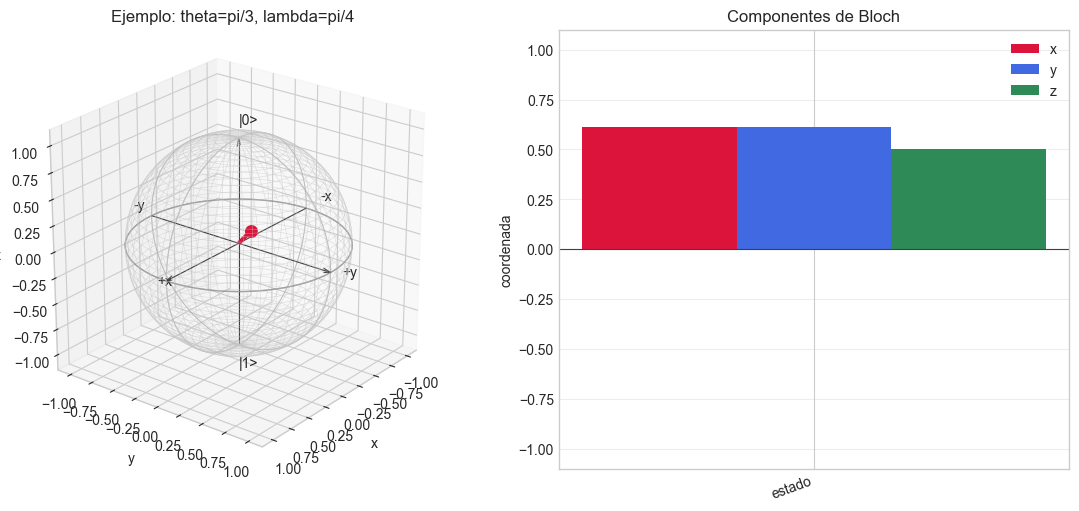
\includegraphics[width=0.92\textwidth]{bloch_estado_general_theta_pi3_lambda_pi4.png}
\caption{Estado general de prueba para \(\theta=\pi/3\) y \(\lambda=\pi/4\). El vector obtenido tiene componentes aproximadamente \((0.6124,0.6124,0.5)\).}
\end{figure}

\begin{figure}[H]
\centering
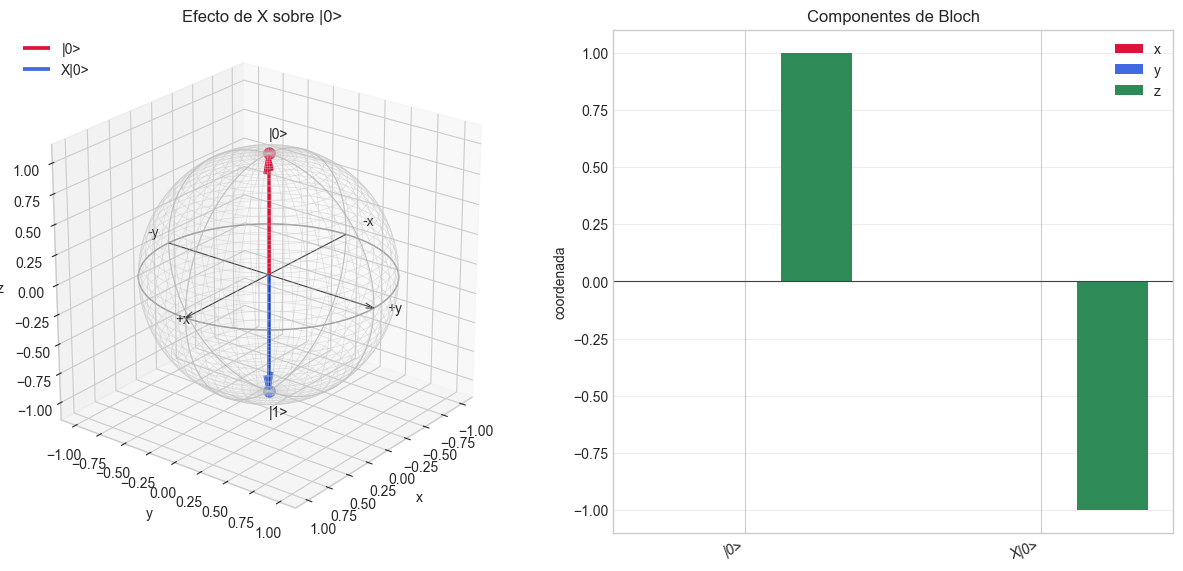
\includegraphics[width=0.92\textwidth]{bloch_compuerta_x_sobre_0.png}
\caption{Efecto de la compuerta \(X\) sobre \(\ket{0}\). El estado pasa del polo norte \((0,0,1)\) al polo sur \((0,0,-1)\).}
\end{figure}

\begin{figure}[H]
\centering
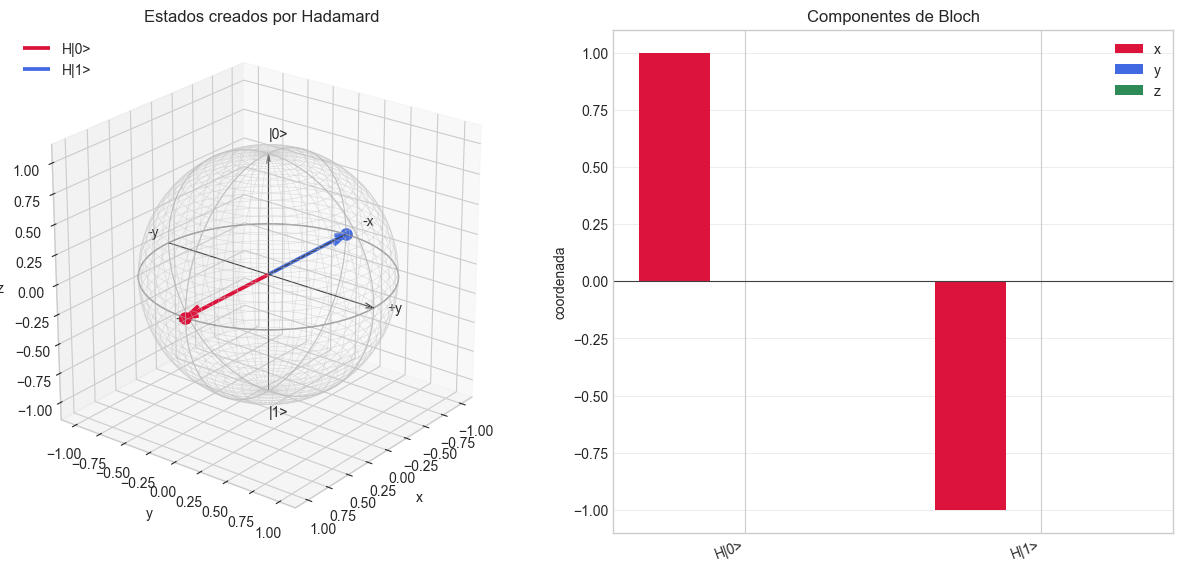
\includegraphics[width=0.92\textwidth]{bloch_hadamard_h0_h1.png}
\caption{Estados generados por la compuerta Hadamard. \(H\ket{0}\) se ubica en \(+x\), mientras que \(H\ket{1}\) se ubica en \(-x\).}
\end{figure}

\begin{figure}[H]
\centering
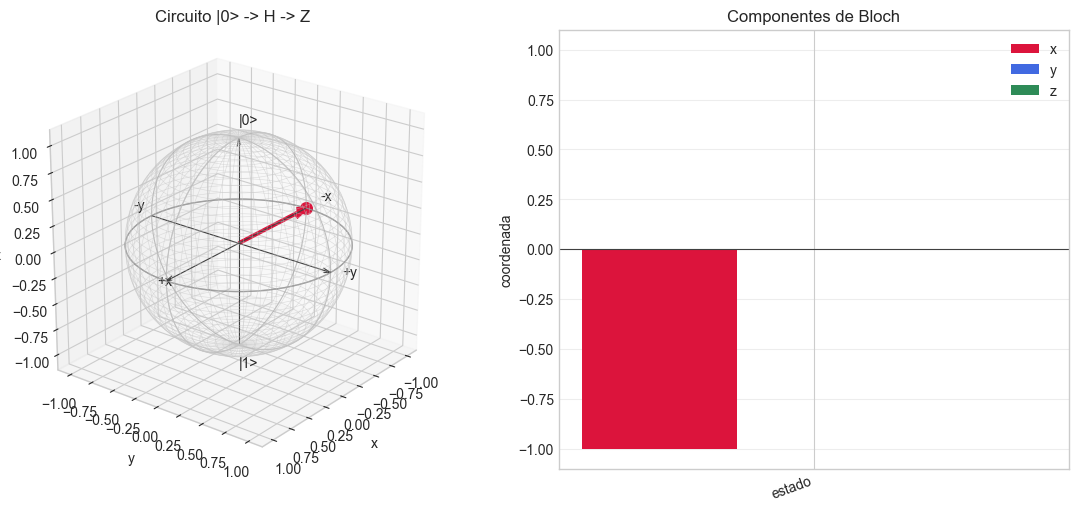
\includegraphics[width=0.92\textwidth]{bloch_circuito_hz.png}
\caption{Circuito \(\ket{0}\rightarrow H\rightarrow Z\). El estado final es \(\frac{\ket{0}-\ket{1}}{\sqrt{2}}\), ubicado en \((-1,0,0)\).}
\end{figure}

\begin{figure}[H]
\centering
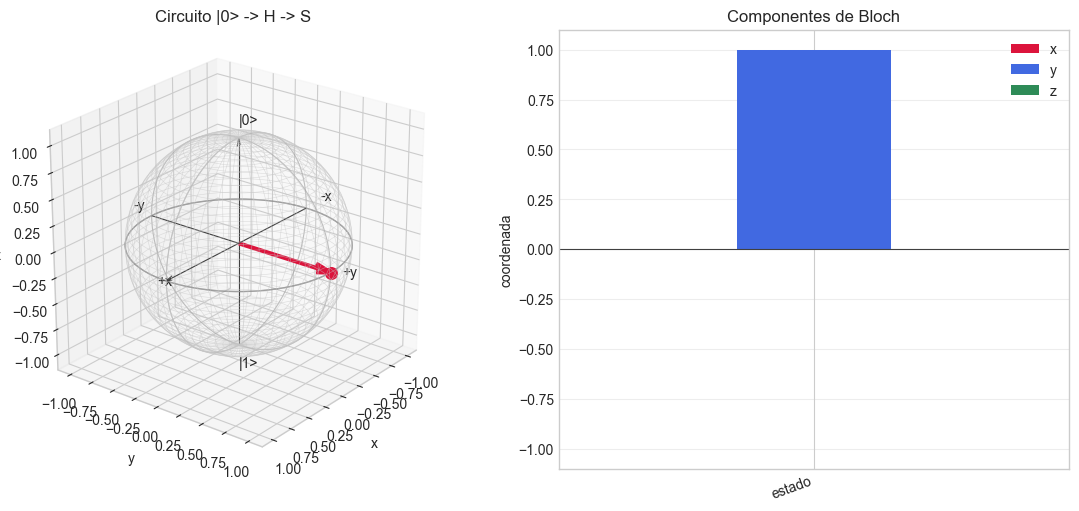
\includegraphics[width=0.92\textwidth]{bloch_circuito_hs.png}
\caption{Circuito \(\ket{0}\rightarrow H\rightarrow S\). El estado final es \(\frac{\ket{0}+i\ket{1}}{\sqrt{2}}\), ubicado en \((0,1,0)\).}
\end{figure}

\begin{figure}[H]
\centering
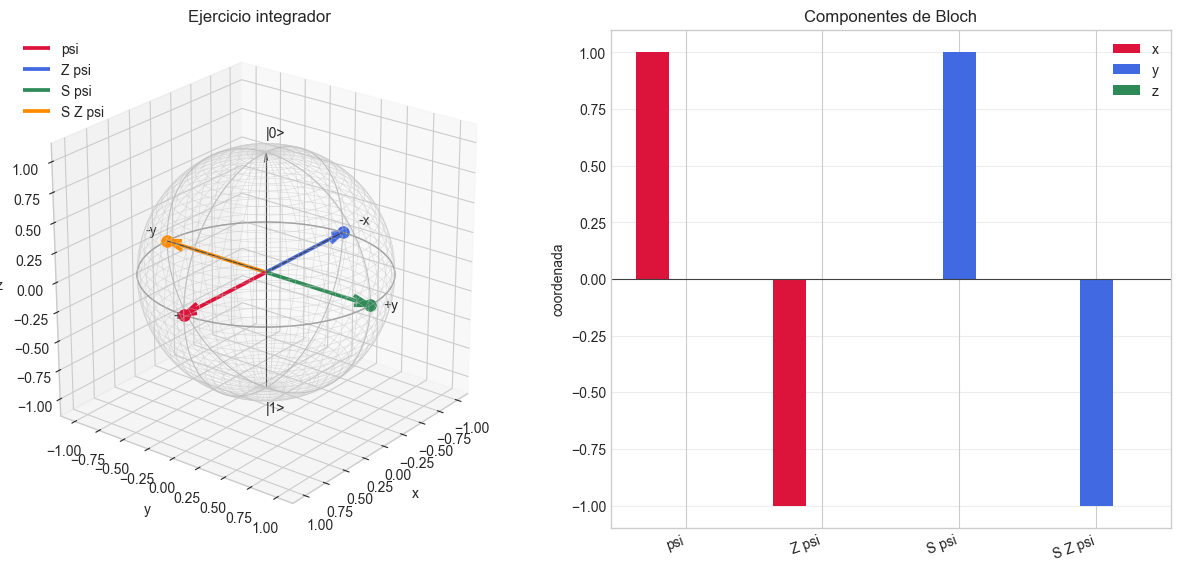
\includegraphics[width=0.92\textwidth]{bloch_ejercicio_integrador.png}
\caption{Comparación del ejercicio integrador. Se observan los estados \(\ket{\psi}\), \(Z\ket{\psi}\), \(S\ket{\psi}\) y \(SZ\ket{\psi}\) en los ejes \(+x\), \(-x\), \(+y\) y \(-y\), respectivamente.}
\end{figure}

Estas visualizaciones confirman que las probabilidades pueden mantenerse iguales mientras cambia la fase relativa del estado. Por esta razón, varios estados tienen \(P(0)=P(1)=1/2\), pero se ubican en direcciones distintas de la esfera de Bloch.

% ==========================================================
\section{Nivel Computacional Opcional: Qiskit}

A continuación se presenta una implementación básica en Qiskit para comprobar los resultados teóricos.

\subsection{Instalación}

\begin{lstlisting}
!pip install qiskit qiskit-aer pylatexenc
\end{lstlisting}

\subsection{Importación de librerías}

\begin{lstlisting}
from qiskit import QuantumCircuit
from qiskit.quantum_info import Statevector
from qiskit.visualization import plot_bloch_multivector
import matplotlib.pyplot as plt
\end{lstlisting}

\subsection{Circuito \texorpdfstring{$\ket{0}\rightarrow H$}{ket 0 H}}

\begin{lstlisting}
qc = QuantumCircuit(1)
qc.h(0)

state = Statevector.from_instruction(qc)

print(state)
display(qc.draw("mpl"))
plot_bloch_multivector(state)
plt.show()
\end{lstlisting}

Resultado teórico:

\[
H\ket{0}=\frac{\ket{0}+\ket{1}}{\sqrt{2}}
\]

Coordenadas:

\[
(x,y,z)=(1,0,0)
\]

\subsection{Circuito \texorpdfstring{$\ket{0}\rightarrow H\rightarrow Z$}{ket 0 H Z}}

\begin{lstlisting}
qc = QuantumCircuit(1)
qc.h(0)
qc.z(0)

state = Statevector.from_instruction(qc)

print(state)
display(qc.draw("mpl"))
plot_bloch_multivector(state)
plt.show()
\end{lstlisting}

Resultado teórico:

\[
ZH\ket{0}=
\frac{\ket{0}-\ket{1}}{\sqrt{2}}
\]

Coordenadas:

\[
(x,y,z)=(-1,0,0)
\]

\subsection{Circuito \texorpdfstring{$\ket{0}\rightarrow H\rightarrow S$}{ket 0 H S}}

\begin{lstlisting}
qc = QuantumCircuit(1)
qc.h(0)
qc.s(0)

state = Statevector.from_instruction(qc)

print(state)
display(qc.draw("mpl"))
plot_bloch_multivector(state)
plt.show()
\end{lstlisting}

Resultado teórico:

\[
SH\ket{0}=
\frac{\ket{0}+i\ket{1}}{\sqrt{2}}
\]

Coordenadas:

\[
(x,y,z)=(0,1,0)
\]

\subsection{Circuito integrador: \texorpdfstring{$\ket{+}\rightarrow Z\rightarrow S$}{ket plus Z S}}

\begin{lstlisting}
qc = QuantumCircuit(1)
qc.h(0)   # Prepara el estado |+>
qc.z(0)   # Aplica la compuerta Z
qc.s(0)   # Aplica la compuerta S

state = Statevector.from_instruction(qc)

print(state)
display(qc.draw("mpl"))
plot_bloch_multivector(state)
plt.show()
\end{lstlisting}

Resultado teórico:

\[
SZ\ket{+}=
\frac{\ket{0}-i\ket{1}}{\sqrt{2}}
\]

Coordenadas:

\[
(x,y,z)=(0,-1,0)
\]

% ==========================================================
\subsection{Figuras generadas con Qiskit}

Las siguientes figuras muestran los circuitos y las visualizaciones de Bloch producidas por Qiskit para los circuitos principales.

\begin{figure}[H]
\centering
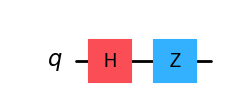
\includegraphics[width=0.38\textwidth]{qiskit_circuito_hz.png}
\caption{Circuito Qiskit para \(\ket{0}\rightarrow H\rightarrow Z\).}
\end{figure}

\begin{figure}[H]
\centering
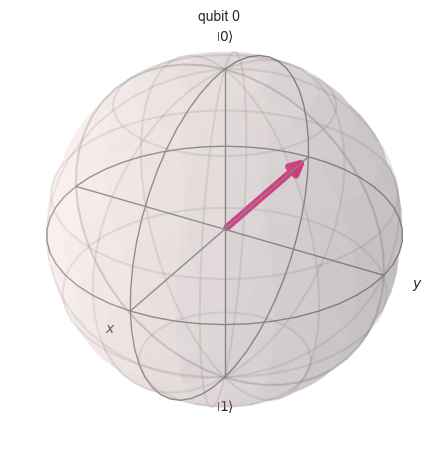
\includegraphics[width=0.55\textwidth]{qiskit_bloch_hz.png}
\caption{Esfera de Bloch generada por Qiskit para el circuito \(ZH\ket{0}\).}
\end{figure}

\begin{figure}[H]
\centering
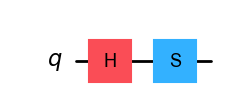
\includegraphics[width=0.38\textwidth]{qiskit_circuito_hs.png}
\caption{Circuito Qiskit para \(\ket{0}\rightarrow H\rightarrow S\).}
\end{figure}

\begin{figure}[H]
\centering
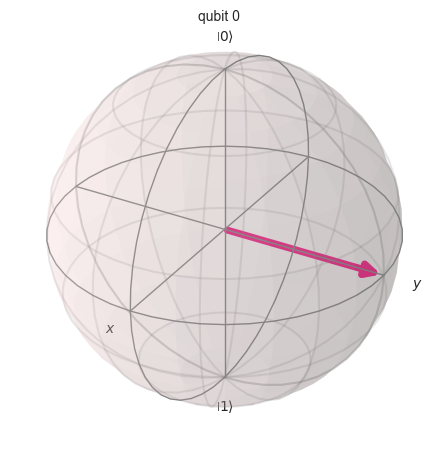
\includegraphics[width=0.55\textwidth]{qiskit_bloch_hs.png}
\caption{Esfera de Bloch generada por Qiskit para el circuito \(SH\ket{0}\).}
\end{figure}

% ==========================================================
\section{Resumen Final}

\begin{table}[h!]
\centering
\begin{tabular}{lll}
\toprule
\textbf{Caso} & \textbf{Estado final} & \textbf{Coordenadas de Bloch} \\
\midrule
\(\ket{0}\) & \(\ket{0}\) & \((0,0,1)\) \\
\(X\ket{0}\) & \(\ket{1}\) & \((0,0,-1)\) \\
\(H\ket{0}\) & \(\dfrac{\ket{0}+\ket{1}}{\sqrt{2}}\) & \((1,0,0)\) \\
\(ZH\ket{0}\) & \(\dfrac{\ket{0}-\ket{1}}{\sqrt{2}}\) & \((-1,0,0)\) \\
\(SH\ket{0}\) & \(\dfrac{\ket{0}+i\ket{1}}{\sqrt{2}}\) & \((0,1,0)\) \\
\(SZH\ket{0}\) & \(\dfrac{\ket{0}-i\ket{1}}{\sqrt{2}}\) & \((0,-1,0)\) \\
\bottomrule
\end{tabular}
\caption{Resumen de estados principales y sus coordenadas en la esfera de Bloch.}
\end{table}

\section{Conclusión}

En este laboratorio se resolvieron ejercicios fundamentales sobre la representación matemática de un qubit, su interpretación geométrica mediante la esfera de Bloch y el efecto de compuertas cuánticas básicas. Se comprobó que las compuertas \(X\), \(Z\), \(S\) y \(H\) modifican el estado cuántico mediante cambios de base, inversión de estados, introducción de fases relativas y generación de superposición.

También se demostró que la fase global no cambia las probabilidades de medición, mientras que la fase relativa sí tiene significado físico, ya que altera la interferencia cuántica. Finalmente, los circuitos propuestos permiten visualizar cómo un qubit puede desplazarse entre distintos puntos de la esfera de Bloch, relacionando el álgebra matricial con la interpretación física del estado cuántico.

\end{document}
